

\begin{figure}
\begin{mdframed}[backgroundcolor=gray!05] 
\begin{scriptsize}

{\large \textbf{Task: Titanic}} \bigskip


Picnics or outdoor lunches are great, especially during summer time. The student association often decides to meet at a rendezvous point and walk towards a picnic place what gives them time to small talk and catch-up with the latest news and gossips. \medskip

For example, students can meet at 
\code{Walter C. Koerner Library, 1958 Main Mall, Vancouver, BC V6T 1Z2} 
and decide to have picnic at 
\code{Jericho Beach, Vancouver, BC}  \medskip

\medskip

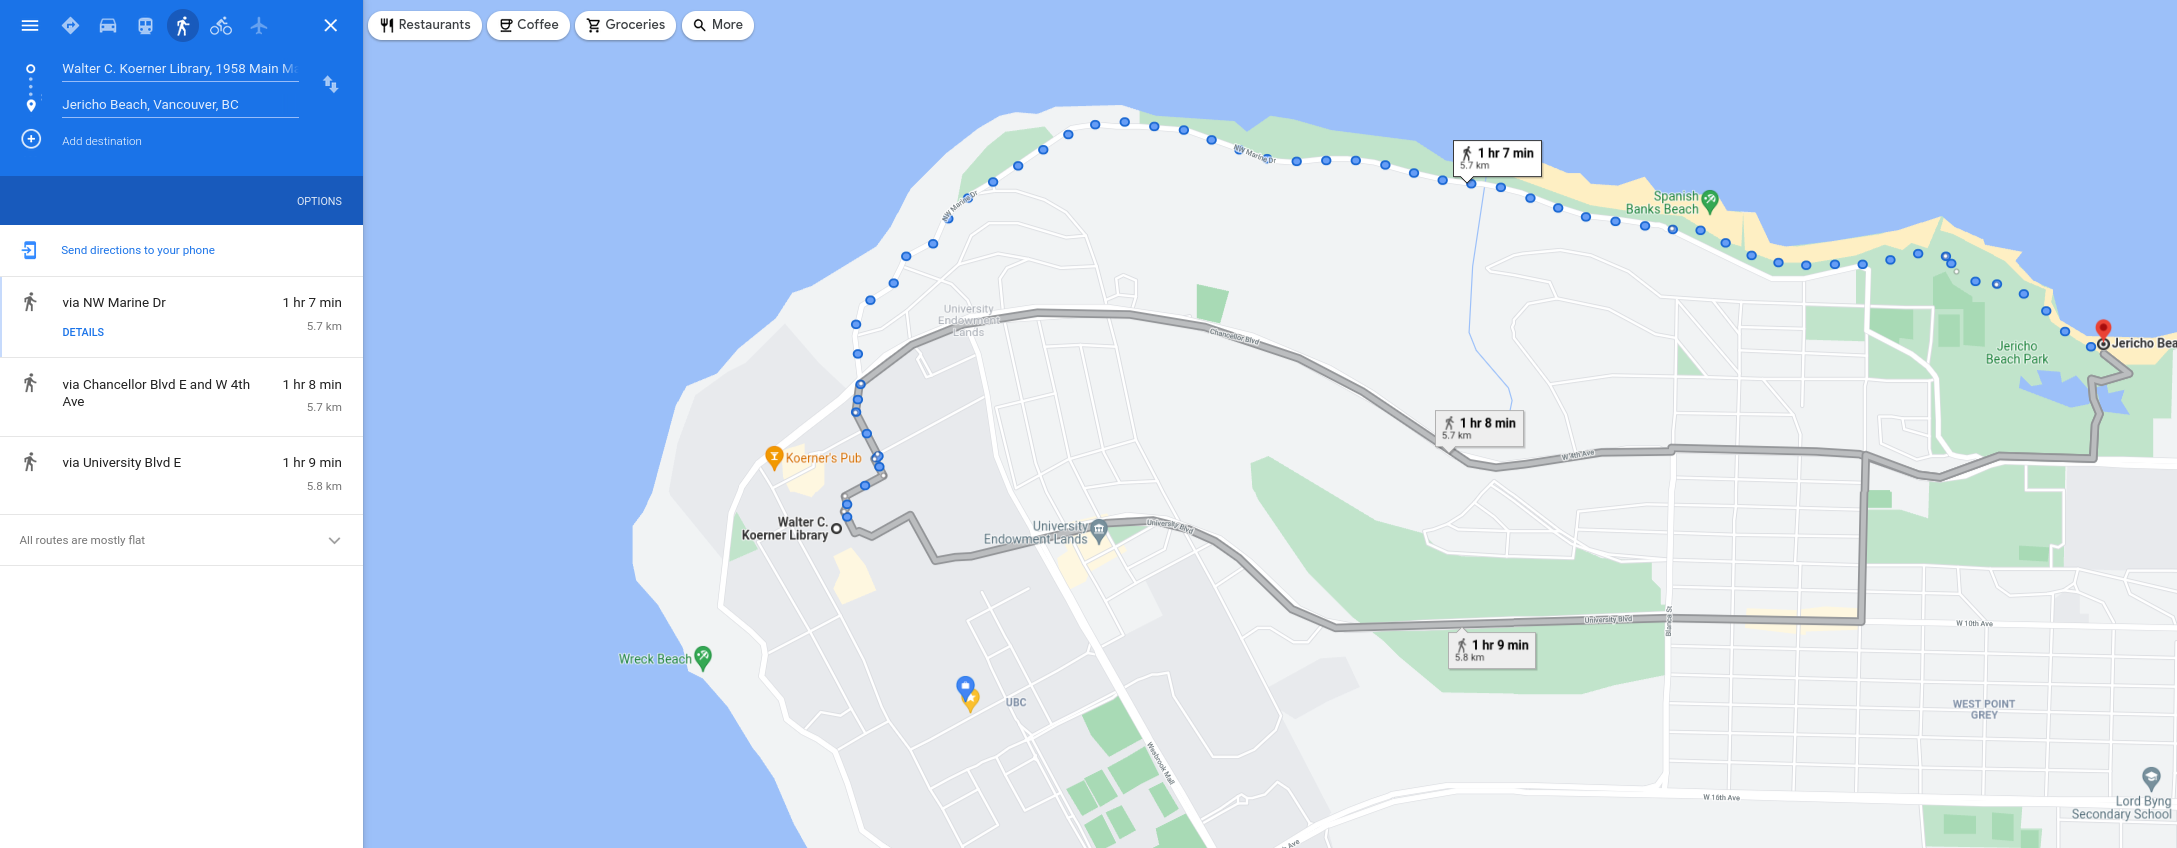
\includegraphics[width=\textwidth]{appendix/cp6/jericho.png}

\medskip


Some students are not happy with walking distances and the student association wants to build a small system that finds the distance between a rendezvous location and a suggested picnic place.  \medskip

Every week, students submit a picnic address and the system should find the place closest to the starting location. \medskip


\begin{center}
\rule{10cm}{0.4pt}
\end{center}

\textbf{Task} \medskip



Given a \code{string}
representing rendezvous address and a \code{list}
of suggested picnic addresses

you must write an algorithm using the \code{geopy}
module to find the closest picnic address. \medskip


Constraints:

\begin{itemize}


    \item  The suggested address must be within 10 km from a meeting location.

    \item  If no suggestion is within 10 km, you should return \code{None}

    \item  There can be invalid addresses either in the meeting place or in the suggestion list

    \item  If two places have the same distance, your solution should return the address that appears first in the list of suggestions 


\end{itemize}

\end{scriptsize}
\end{mdframed}
\end{figure}
  


\begin{figure}
\begin{mdframed}[backgroundcolor=gray!05] 
\begin{scriptsize}



\textbf{Input} 


\begin{python}
rendezvous_address = "1958 Main Mall, Vancouver, BC V6T 1Z2"
suggestions = ["Spanish Banks West Concession"]
\end{python}

\textbf{Output}


\begin{python}
expected = "Spanish Banks West Concession"
\end{python}

\textbf{Explanation} \medskip


There is a single suggestion. The distance between the rendezvous address and the suggested location is less than the max allowed distance. Therefore, the expected output is \code{Spanish Banks West Concession}

    


\begin{center}
\rule{10cm}{0.4pt}
\end{center}



\textbf{Input}

\begin{python}
rendezvous_address = "1958 Main Mall, Vancouver, BC V6T 1Z2"
suggestions = [
    "Spanish Banks West Concession",
    "Museum of Anthropology University of British Columbia"
]
\end{python}

\textbf{Output}


\begin{python}
expected = "Museum of Anthropology University of British Columbia"
\end{python}

\textbf{Explanation} \medskip


The distance between the meeting place and \code{Spanish Banks} is 5.7km.  The distance between the meeting place and the \code{Museum of Anthropology} is 600m. The museum is closer, hence it should be the expected output. 

    


\begin{center}
\rule{10cm}{0.4pt}
\end{center}
  


\textbf{Resources}

\begin{itemize}
    \item \href{link}{}
    \item \href{link}{}
    \item \href{link}{}
    \item  \href{link}{}
    \item  \href{link}{}
    \item  \href{link}{}
    \item  \href{link}{}
    \item  \href{link}{} 
    \item  \href{link}{}
    \item  \href{link}{}
    \item  \href{link}{}
\end{itemize}

\end{scriptsize}
\end{mdframed}
\caption{Description for the Titanic task}
\end{figure}

    